\documentclass[border=4pt]{standalone}
\usepackage{lmodern}
\usepackage[T1]{fontenc}
\usepackage{amsmath,amssymb}
\usepackage{tikz}
\usetikzlibrary{shapes.geometric, arrows.meta, positioning, fit, backgrounds, calc}
\begin{document}
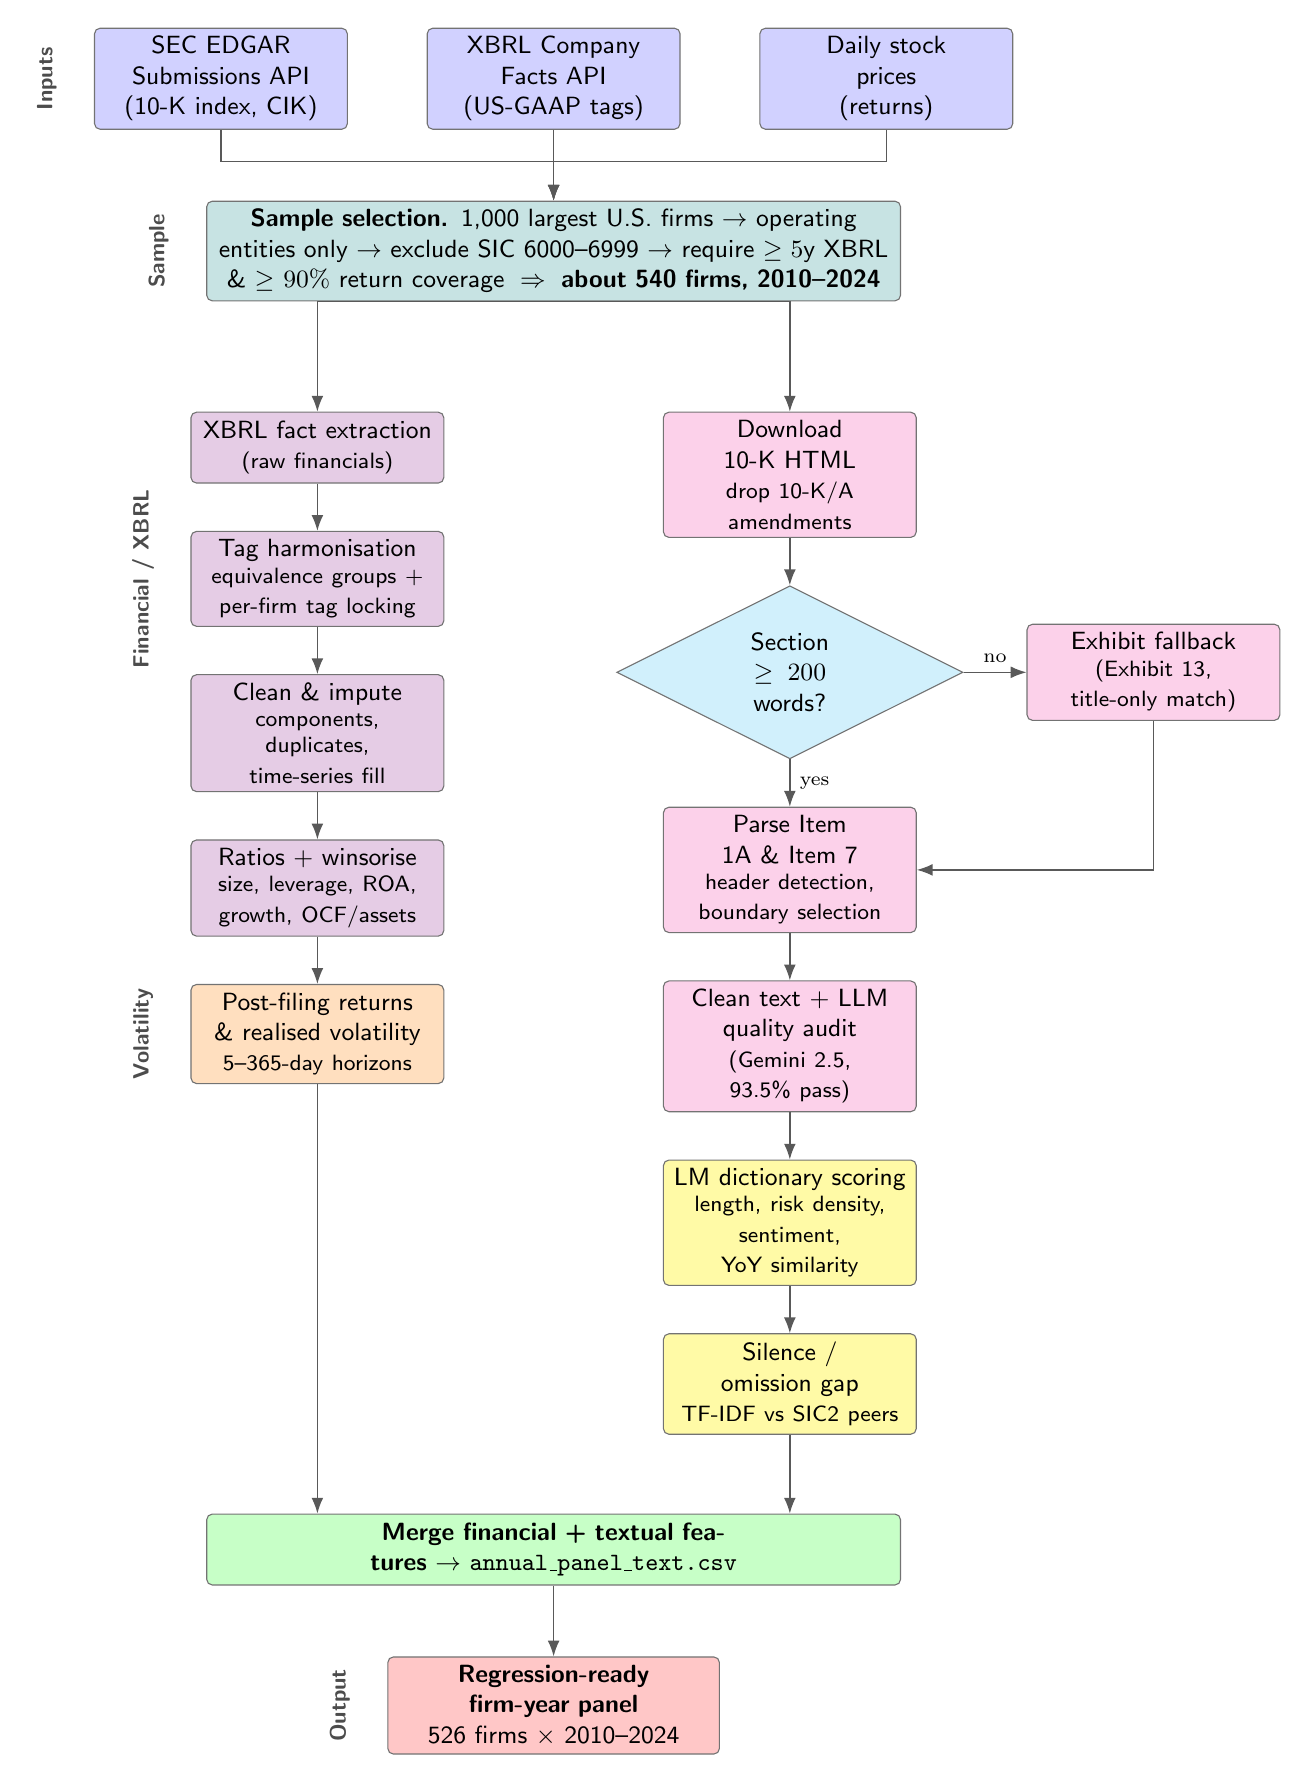
\begin{tikzpicture}[
    font=\sffamily\small,
    >={Latex[length=2mm]},
    node distance=6mm,
    box/.style={rounded corners=2pt, draw=black!55, line width=0.4pt,
                align=center, text width=30mm, minimum height=9mm,
                inner sep=3pt},
    src/.style={box, fill=blue!18},
    samp/.style={box, fill=teal!22, text width=86mm},
    fin/.style={box, fill=violet!20},
    vol/.style={box, fill=orange!25},
    txt/.style={box, fill=magenta!18},
    feat/.style={box, fill=yellow!35},
    dec/.style={diamond, aspect=2, draw=black!55, line width=0.4pt,
                fill=cyan!18, align=center, inner sep=1pt, text width=22mm},
    outbox/.style={box, fill=red!22, text width=40mm},
    merge/.style={box, fill=green!22, text width=86mm},
    arr/.style={->, draw=black!65, line width=0.5pt},
    stage/.style={rotate=90, anchor=center, font=\sffamily\bfseries\footnotesize,
                  text=black!70},
]

% ---- Sources (inputs) ----
\node[src] (s1) {SEC EDGAR\\ Submissions API\\ (10-K index, CIK)};
\node[src, right=10mm of s1] (s2) {XBRL Company\\ Facts API\\ (US-GAAP tags)};
\node[src, right=10mm of s2] (s3) {Daily stock\\ prices\\ (returns)};

% ---- Sample selection (spans width) ----
\node[samp, below=9mm of s2] (sel)
  {\textbf{Sample selection.} 1{,}000 largest U.S.\ firms
   $\rightarrow$ operating entities only $\rightarrow$ exclude SIC 6000--6999
   $\rightarrow$ require $\geq 5$y XBRL \& $\geq 90\%$ return coverage
   \;$\Rightarrow$\; \textbf{about 540 firms, 2010--2024}};

% ---- Financial branch (left) ----
\node[fin, below=14mm of sel.south, xshift=-30mm] (f1)
  {XBRL fact extraction\\ \footnotesize(raw financials)};
\node[fin, below=of f1] (f2)
  {Tag harmonisation\\ \footnotesize equivalence groups +\\ per-firm tag locking};
\node[fin, below=of f2] (f3)
  {Clean \& impute\\ \footnotesize components, duplicates,\\ time-series fill};
\node[fin, below=of f3] (f4)
  {Ratios + winsorise\\ \footnotesize size, leverage, ROA,\\ growth, OCF/assets};
\node[vol, below=of f4] (f5)
  {Post-filing returns\\ \& realised volatility\\ \footnotesize 5--365-day horizons};

% ---- Text branch (right) ----
\node[txt, below=14mm of sel.south, xshift=30mm] (t1)
  {Download 10-K HTML\\ \footnotesize drop 10-K/A amendments};
\node[dec, below=of t1] (td)
  {Section\\ $\geq 200$\\ words?};
\node[txt, right=8mm of td] (tx)
  {Exhibit fallback\\ \footnotesize (Exhibit 13,\\ title-only match)};
\node[txt, below=of td] (t2)
  {Parse Item 1A \& Item 7\\ \footnotesize header detection,\\ boundary selection};
\node[txt, below=of t2] (t3)
  {Clean text + LLM\\ quality audit\\ \footnotesize (Gemini 2.5, 93.5\% pass)};
\node[feat, below=of t3] (t4)
  {LM dictionary scoring\\ \footnotesize length, risk density,\\ sentiment, YoY similarity};
\node[feat, below=of t4] (t5)
  {Silence / omission gap\\ \footnotesize TF-IDF vs SIC2 peers};

% ---- Merge + output ----
\node[merge, below=10mm of t5.south, anchor=north, xshift=-30mm] (mg)
  {\textbf{Merge financial + textual features} $\rightarrow$
   \texttt{annual\_panel\_text.csv}};
\node[outbox, below=9mm of mg] (out)
  {\textbf{Regression-ready firm-year panel}\\ 526 firms $\times$ 2010--2024};

% ---- Arrows: sources -> selection ----
\draw[arr] (s1.south) -- ($(s1.south)+(0,-4mm)$) -| (sel.north);
\draw[arr] (s2.south) -- (sel.north);
\draw[arr] (s3.south) -- ($(s3.south)+(0,-4mm)$) -| (sel.north);

% ---- Selection -> branch heads ----
\draw[arr] (sel.south) -| (f1.north);
\draw[arr] (sel.south) -| (t1.north);

% ---- Financial chain ----
\draw[arr] (f1) -- (f2);
\draw[arr] (f2) -- (f3);
\draw[arr] (f3) -- (f4);
\draw[arr] (f4) -- (f5);

% ---- Text chain ----
\draw[arr] (t1) -- (td);
\draw[arr] (td) -- node[above, font=\scriptsize] {no} (tx);
\draw[arr] (tx.south) |- (t2.east);
\draw[arr] (td) -- node[right, font=\scriptsize] {yes} (t2);
\draw[arr] (t2) -- (t3);
\draw[arr] (t3) -- (t4);
\draw[arr] (t4) -- (t5);

% ---- Branches -> merge ----
\draw[arr] (f5.south) -- (f5.south |- mg.north);
\draw[arr] (t5.south) -- (t5.south |- mg.north);
\draw[arr] (mg) -- (out);

% ---- Stage labels (swimlane-style, left margin) ----
\node[stage] at ($(s1.west)+(-6mm,0)$) {Inputs};
\node[stage] at ($(sel.west)+(-6mm,0)$) {Sample};
\node[stage] at ($(f2.west)+(-6mm,0)$) {Financial / XBRL};
\node[stage] at ($(f5.west)+(-6mm,0)$) {Volatility};
\node[stage] at ($(out.west)+(-6mm,0)$) {Output};

\end{tikzpicture}
\end{document}
